\chapter{Metodologia}

Introduzir o capitulo de Metodologia - sobre o que falaremos.

\section{Termo de Abertura do Projeto - TAP}

Trazer o TAP.

\section{Estrutura Analítica do Projeto (EAP)}

Trazer e explicar a EAP do projeto - com respeito aos pontos de controle.

\section{Comunicação}

Explicar o método que o time utilizou para se comunicar - ferramentas, reuniões, etc.

\section{Custos}

Explicar o método que utilizaremos para gerenciar os custos.

\section{Tempo}

Para gerenciar o tempo no projeto, foi utilizado como base os processos
de gerenciamento de tempo do \cite{pmbok2012}.

A partir do escopo do projeto, foi feito o cronograma inicial utilizando o software \textit{Gantter} armazenado no \textit{Google Drive} para que todos os membros do projeto
possam acessá-lo e assim fazer o controle do cronograma.

\subsection{Cronograma}

O cronograma encontra-se no Apêndice \ref{schedule_appendix}.

\section{Recursos Humanos}

O projeto foi dividido em três subprojetos, que são: Processamento de Sinais e Monitoramento,
Projeto Estrutural e Controle e Alimentação. Dentro dos subprojetos a equipe
técnica foi dividida de acordo com a demanda de cada área e levando em conta o
conhecimento prévio de cada integrante, bem como o seu interesse de atuação. Os
subprojetos serão gerenciados por um Gerente Geral, um Gerente de Qualidade e
um Gerente de Produto.
Abaixo tem-se uma breve descrição do setor de gerenciamento e dos subprojetos,
e também os integrantes que compõem cada área. É válido ressaltar que a
distribuição e responsabilidades de cada equipe poderão sofrer mudanças no
decorrer do projeto para melhor atender as necessidades de cada área e
consequentemente obter um melhor desempenho dos integrantes e o êxito do projeto.

\subsection{Gerenciamento}

\textbf{Gerente Geral:} responsável pelo planejamento, pela organização e pelo controle das atividades desempenhadas pelos integrantes de cada equipe, bem como pela assessoria a cada subprojeto e atualização de informações pertinentes ao projeto como um todo.
\\Responsável: Afonso Delgado

\textbf{Gerente de Qualidade:} responsável por fiscalizar a qualidade do que está sendo produzido fazendo uma análise crítica da produção, de maneira a obter uma maior confiabilidade, produtividade, redução de custos e otimização dos processos realizados por cada equipe.
\\Responsável: Dylan Guedes

\textbf{Gerente de Produto:} responsável por prestar suporte a todos os subprojetos, visando aperfeiçoar a capacidade de produção dos integrantes do projeto, focando na qualidade da entrega final, impedindo, assim,  que fatores alheios atrapalhem a experiência do cliente com o produto final.
\\Responsável: Rafael Amado

\subsection{Subprojetos}

\textbf{Processamento de Sinais e Monitoramento:} responsável pela aquisição de sinais vitais do paciente,
tratamento de sinais, amplificação e conversão, transmissão e apresentação de
dados via notificações web e mobile.
\\Responsáveis: Dylan Guedes, Wilton Rodrigues, Tiago Assunção, Gustavo Cavalcante e Afonso Delgado.

\textbf{Projeto Estrutural:} responsável pelo projeto estrutural da cadeira, testes
do sistema estrutural, simulações e construção da cadeira.
\\Responsáveis: Nivaldo Lopo, Rafael Amado, Lucas Oliveira.

\textbf{Controle e Alimentação:} responsável por dimensionamento dos motores utilizados,
baterias e sistemas de movimentação e ativação dos motores (controle por
joystick e driver para motores).
\\Responsáveis: Lunara Martins, Mariana Andrade, Cesar Marques, Johnson Andrade e Felipe Costa.

Na Figura \ref{flux_rh} é apresentada a estrutura de alocação de recursos humanos da equipe.


\begin{figure}[h]
    \centering
    \label{flux_rh}
    \includegraphics[keepaspectratio=true,scale=0.18]{figuras/flux_rh.eps}
    \caption{Estrutura de alocação de recursos humanos.}
\end{figure}

\subsection{Tarefas}

Nesta seção visa detalhar o que foi feito por cada um dos membros do projeto no PC1.

\begin{table}[h]
  \begin{center}
  \caption{\label{tarefas}Tarefas realizadas durante o PC1 pelo subsistema PSM.}
  \begin{tabular}{|l|l|l|l|}
  \hline
  \textbf{Membro} & \textbf{Atividade} & \textbf{Data} \\ \hline\hline
  Gustavo & Criar o cronograma & 24/03 \\ \hline
   & Elicitação de requisitos & 25/03 \\ \hline
   & Definição da arquitetura PSM & 25/03 \\ \hline
   & Finalizar seção do tempo & 28/03 \\ \hline
   & Subseção de tarefas & 31/03\\ \hline
  Wilton & Levantamento de requisitos & 25/03 \\ \hline
   & Definição da arquitetura PSM & 25/03 \\ \hline
  Dylan Guedes & Definição da arquitetura do PSM & 29/03\\ \hline
   & Revisão do Relatório & 31/03 \\ \hline
  Tiago & Definição da arquitetura geral & 25/03 \\ \hline
   & Revisão da metodologia & 26/03 \\ \hline
   & Construção do TAP & 27/03 \\ \hline
  Afonso & Definição arquitetura de PSM & 26/03 \\ \hline
   & Escrita de capítulo de introdução e problemática & 27/03 \\ \hline
   & Definição dos meios de comunicação & 27/03 \\ \hline
   & Definição de requisitos do projeto & 26/03 \\ \hline
  \end{tabular}
  \end{center}
\end{table}

\begin{table}[h]
  \begin{center}
  \caption{\label{tarefas}Tarefas realizadas durante o PC1 pelo subsistema PE.}
  \begin{tabular}{|l|l|l|l|}
  \hline
  \textbf{Membro} & \textbf{Atividade} & \textbf{Data} \\ \hline\hline
  Lucas & Definição da arquitetura PE & 25/03 \\ \hline
   & Revisar metodologia & 26/03 \\ \hline
   & Revisar recursos humanos & 27/03 \\ \hline
  Rafael Amado  & Levantamento de requisitos  & 26/03 \\ \hline
   & Elaboração do TAP & 26/03 \\ \hline
   & Mapeamento de peças estruturais & 26/03 \\ \hline
   & Levantamento de riscos & 26/03 \\ \hline
  Nivaldo Lopo  & Busca de possiveis materiais no galpão & 27/03 \\ \hline
   & Revisão dos niveis dos riscos da estrutura & 27/03 \\ \hline
   & Elaboração do EAP & 27/03 \\ \hline
  \end{tabular}
  \end{center}
\end{table}

\begin{table}[h]
  \begin{center}
  \caption{\label{tarefas}Tarefas realizadas durante o PC1 pelo subsistema CeA.}
  \begin{tabular}{|l|l|l|l|}
  \hline
  \textbf{Membro} & \textbf{Atividade} & \textbf{Data} \\ \hline\hline
  Cesar Júnior & Elaboração texto arquitetura  & 27/03 \\ \hline
   & Definição dos requisitos de projeto & 28/03 \\ \hline
  Lunara Martins & Pesquisas sobre alimentação da cadeira & 23/03 \\ \hline
   & Elaboração dos riscos do projeto & 27/03 \\ \hline
   & Revisão de requisitos de CeA & 28/03 \\ \hline
   & Revisão do dimensionamento do motor & 29/03 \\ \hline
  Felipe Costa & Definição de arquitetura CeA & 28/03 \\ \hline
   & Levantamento e classificação dos riscos & 29/03 \\ \hline
  Johnson Andrade & Definição arquitetura de Controle & 28/03 \\ \hline
   & Elaboração do texto de arquitetura  & 28/03 \\ \hline
   & Levantamento e classificação de riscos  & 29/03 \\ \hline
  Mariana Andrade & Texto de alocação de recursos humanos & 27/03 \\ \hline
   & Elaboração de requisitos para CeA & 30/03 \\ \hline
   & Dimensionamento do motor & 30/03 \\ \hline
   & Revisão de riscos do projeto & 29/03 \\ \hline
  \end{tabular}
  \end{center}
\end{table}

\section{Requisitos}

Explicar como gerenciaremos os requisitos do projeto.

\section{Riscos}

Explicar como gerenciaremos e mitigaremos os riscos.

\section{Desenvolvimento do Relatório}

A confecção do relatório será dividida em dois fluxos - um geral, onde o
conteúdo será escrito e revisado, e a implantação no relatório, onde um
membro que domine \LaTeX\ e
Git\footnote{\url{https://git-scm.com/}} transcreverá o conteúdo para o
relatório final.

\subsection{Fluxo 1 - Criação do conteúdo}

\begin{figure}[H]
  \centering
    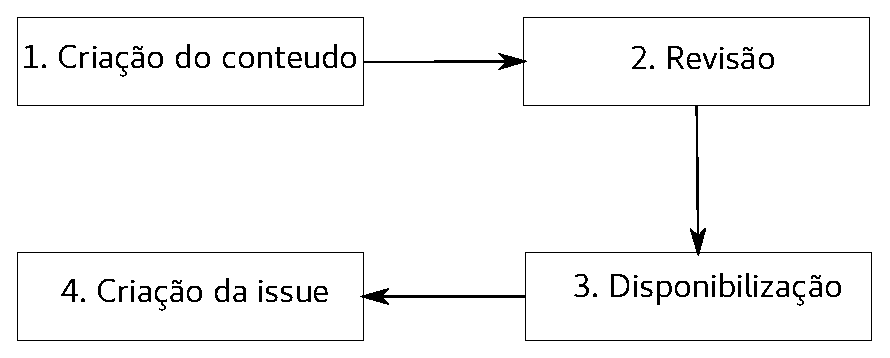
\includegraphics[width=\textwidth]{figuras/fluxo1.eps}
  \caption{Fluxo 1 - Criação do conteúdo.}
  \label{fig:fluxo1}
\end{figure}

\begin{enumerate}
  \item O conteúdo é escrito, de maneira formatada e com referências;
  \item O conteúdo é revisado pelo seu autor, que corrigirá defeitos encontrados;
  \item O autor disponibiliza o conteúdo em algum meio acessível pelos outros membros;
  \item O autor cria uma \textit{issue} no repositório do
    relatório\footnote{\url{https://github.com/CadeiraCuidadora/relatorio}}, explica brevemente
    o conteúdo criado, e disponibiliza o \textit{link} para o conteúdo. A \textit{issue} deverá ser associada a \textit{label} de relatório.
\end{enumerate}

\subsection{Fluxo 2 - Implantação no Relatório}

\begin{enumerate}
  \item Um membro que domine Git e \LaTeX\ encontra uma \textit{issue} que deseja
  implantar no relatório;
  \item Revisa o conteúdo, e o transcreve para o relatório;
  \item Relata na \textit{issue} associada se algum problema ocorreu, ou se terminou a transcrição;
  \item Cria um \textit{merge request} para a \textit{branch master} no repositório;
  \item Outro membro revisa o \textit{merge request}, e aceita ou relata as correções a serem feitas.
\end{enumerate}

